\documentclass[border=5mm]{standalone}
\usepackage{amsmath}
\usepackage{tikz}

\begin{document}

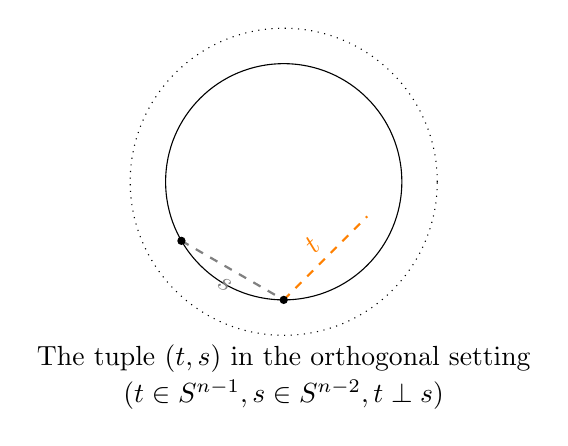
\begin{tikzpicture}[scale=1.5]
    % Draw the sphere
    \draw (0,0) circle (1);
    \draw[dotted] (0,0) circle (1.3); % Dashed circle representing the 2-sphere

    % Define the points
    \coordinate (A) at (-90:1);
    \coordinate (B) at (210:1);

    % Draw the tangent vector t
    \draw[orange, thick, dashed] (A) -- node[midway, above, sloped] {$t$} ++(45:1);

    % Draw the normal vector s
    \draw[gray, thick, dashed] (B) -- node[midway, below, sloped] {$s$} ++(-30:1);

    % Mark the points
    \fill (A) circle (1pt);
    \fill (B) circle (1pt);

    \node at (0,-1.5) {The tuple $(t, s)$ in the orthogonal setting};
    \node at (0,-1.8) {$(t \in \mathbb{S}^{n-1}, s \in \mathbb{S}^{n-2}, t \perp s)$};

\end{tikzpicture}

\end{document}